%% Supplementary material for the IEEE T-ITS revision.
%% Everything here was part of the Elsevier version of the manuscript and is
%% carried over verbatim; it lives in this document so that the main paper stays
%% within the T-ITS page limit.

\documentclass[journal]{IEEEtran}

\usepackage[numbers,sort&compress]{natbib}
\usepackage{graphicx}
\usepackage{amsmath}
\usepackage{amssymb}
\usepackage{booktabs}
\usepackage{siunitx}
\usepackage{array}
\usepackage[caption=false]{subfig}
\usepackage{algorithm}
\usepackage{algpseudocode}
\usepackage{enumitem}
\usepackage{url}
\usepackage[hidelinks]{hyperref}

\begin{document}

\title{Supplementary Material for\\ ``Learning to Route Electric Trucks Under\\ Operational Uncertainty''}
\author{Anonymous authors}
\markboth{Supplementary material}{}
\maketitle

\section{Extended Related Work}

\subsection{Classic Optimization Approaches}

Optimization-based approaches form the analytical backbone of electric truck routing by embedding charging decisions, uncertainty, and energy-feasibility constraints directly into mathematical formulations. A common objective in this direction is to preserve operational realism by explicitly coupling routing and charging, often at the expense of computational tractability. Stochastic formulations illustrate this direction by separating route design from charging recourse under uncertainty. For example, \cite{SPINELLI2026105480} models customer sequencing in a first stage and charging decisions in a second stage to minimize expected route duration. Robust optimization provides a complementary perspective for freight applications, where battery depletion is operationally unacceptable, as shown by \cite{AMIRI2023109108} for heavy-duty electric trucks under uncertain energy consumption. Conic and mixed-integer formulations further increase modeling fidelity by incorporating realistic energy-consumption drivers such as road conditions, vehicle dynamics, payload, and distance~\citep{WANG2024123407}. Although these models offer strong interpretability and disciplined feasibility control, their execution time grows rapidly with fleet size, uncertainty, and physical realism, motivating decomposition~\citep{ziyan2025} and approximation~\cite{lara_electric_2020} techniques to improve scalability in multistage settings using Stochastic Dual Dynamic Programming (SDDP). 
% Overall, optimization-based methods provide a principled foundation for electric truck routing, but their cost can become prohibitive when large fleets, detailed physics, or real-time decisions are involved.
Optimization-based methods provide a principled foundation for eTFRP, but their computational cost can become prohibitive when large fleets, detailed charging behavior, and uncertainty must be modeled jointly. In contrast, our approach preserves these operational interactions in a learning-compatible formulation that supports faster decision-making and direct comparison with optimization baselines within a common simulation setting.


\subsection{Metaheuristic and Population-Based Approaches}

To reduce the computational burden of high-fidelity stochastic and robust formulations, many studies adopt metaheuristics that scale better to larger problem instances while accommodating charging-related constraints. A common strategy is to integrate routing and charging decisions within flexible search procedures, including methods that jointly optimize trip time, cost, charging schedules, and service constraints \citep{https://doi.org/10.1049/pel2.12555}. Variable-neighborhood search (VNS) and other hybrid improvement heuristics have also been used to address capacitated electric truck routing while targeting cost and distance objectives \citep{euchi_hybrid_2023}. When dynamic conditions are present, evolutionary and memetic methods become especially attractive because they can combine local search with adaptive diversification mechanisms to handle mid-route recharging and newly arriving requests \citep{dong_dynamic_2023,https://doi.org/10.1155/2021/6635749}. Bilevel ant-colony optimization (ACO) approaches provide another perspective by separating customer sequencing from charging-feasibility repair \citep{9409782}. 
Overall, metaheuristics offer a practical balance between flexibility and computational speed, but their performance is often instance- and tuning-dependent, and their treatment of uncertainty and feasibility is typically embedded in problem-specific repair logic. In contrast, our method encodes operational feasibility directly into the decision process via a rule-based action mask and systematically evaluates performance in multiple stochastic settings of varying size.

\subsection{Reinforcement Learning Approaches}

Here, the research progress on RL-based routing is split into advances in classic routing (VRP and TSP) and its electric vehicle extension (eVRP).

\subsubsection{RL for classical routing problems}

Recent progress in RL for routing has been driven by learned heuristics that enable combinatorial search across instances and fast decision-making at deployment time, both of which are essential for freight operations that require frequent replanning. A central paradigm is the constructive encoder--decoder policy, in which routes are built sequentially using attention mechanisms. The attention model of \cite{kool2018attention} demonstrates that such policies can achieve strong performance with policy-gradient training and rollout-based baselines, while related work showed that a single policy can learn near-optimal routing decisions over broad instance distributions using only reward signals and feasibility rules \citep{NEURIPS2018_9fb4651c}. Subsequent research has focused on improving training stability and generalization through diverse rollouts and symmetry-aware regularization, leveraging the invariances of routing problems to improve robustness beyond the training distribution \citep{Sym-NCO}. Beyond constructive policies, learning-to-search approaches have sought to emulate classical improvement heuristics by learning local search moves directly; for example, \cite{NEURIPS2023_9bae70d3} learns flexible transformations and uses guided exploration to navigate complex search spaces. More broadly, these studies show that RL can serve as an effective framework for routing, particularly when fast inference and repeated decision-making are required.


\subsubsection{RL for electric vehicle routing}

Building on advances in learning-based routing, recent studies have extended RL to settings where routing decisions must remain energy-feasible and explicitly account for charging actions. One stream adapts constructive attention-based policies to eVRP variants, such as eVRP-TW (with Time-Windows), demonstrating that end-to-end neural policies can handle charging and time-window constraints with competitive performance on benchmark instances \citep{lin2025,10608117}. A second stream increases modeling realism by incorporating vehicle dynamics, road conditions, and charging losses into the learning process through transformer-based or attention-enhanced architectures tailored to eVRP settings \citep{TANG2023121711,11016767}. A third stream focuses on uncertainty and safety, which are especially important in electric freight because battery depletion carries substantial operational risk; for example, safe RL formulations have been proposed for dynamic stochastic settings with uncertain demand and energy consumption \citep{BASSO2022102496}. Hybrid and multi-agent approaches further broaden the design space by combining RL with heuristic selection, charging-repair mechanisms, or explicit modeling of agent interactions and grid-related considerations \citep{lin2022,10310266,ALQAHTANI2022122626}. 

Overall, RL-based electric vehicle routing research has developed rapidly, but most existing methods address only part of the problem addressed here. Prior studies typically focus on single-vehicle or unrealistic eVRP settings, simplified charging assumptions, or isolated aspects such as safety, heuristic selection, or multi-agent coordination. By contrast, the proposed method is designed for fleet-level electric truck routing with shared charging resources, combines explicit feasibility-aware action selection with a graph-based learning architecture, and evaluates these decisions under uncertainty within a common benchmarking environment that also includes heuristic and optimization baselines.

% \subsubsection{classic optimization approaches for eVRP}
% % classic optimization appraoches for eVRP

% \cite{SPINELLI2026105480} as a two-stage stochastic mixed-integer second-order cone model, where the first stage determines the sequences of customers to be visited, and the second stage incorporates charging activities. The objective is to minimize the expected total duration of the routes, composed by travel times and recharging operations

% \cite{AMIRI2023109108} Introduces a new robust mathematical model for the eVRP with Heavy-duty Battery Electric Trucks to handle the energy consumption uncertainty in the short-haul delivery problems

% \cite{WANG2024123407} ropose an energy consumption model that accounts for realistic driving dynamics, road conditions, weight, and distances. Integrating this model into the routing problem, we address energy consumption uncertainty using second-order cone mixed-integer programming

% \cite{ziyan2025} 

% \cite{lara_electric_2020} address the long-term planning of electric power infrastructure under uncertainty. We propose a Multistage Stochastic Mixed-integer Programming formulation that optimizes the generation expansion to meet the projected electricity demand over multiple years while considering detailed operational constraints, intermittency of renewable generation, power flow between regions, storage options, and multiscale representation of uncertainty (strategic and operational). To be able to solve this large-scale model, which grows exponentially with the number of stages in the scenario tree, we decompose the problem using Stochastic Dual Dynamic Integer Programming (SDDiP)

% \subsubsection{metaheuristic for eVRP}
% \cite{https://doi.org/10.1049/pel2.12555} rovides a Bat optimisation technique to reduce trip time and costs while taking into account customer service requests and EV charging schedules. Taking into account battery capacity, charging duration, and delivery/pickup needs
% \cite{euchi_hybrid_2023} Hybrid Variable Neighbourhood Search (HVNS)” is proposed to solve the CE-VRP. The results provide indications on the ideal size of the fleet, and on the total distance traveled while minimizing the associated costs. 

% \cite{https://doi.org/10.1155/2021/6635749} proposes an adaptive memetic algorithm, where a special encoding strategy, an adaptive local search operator, and an economical random immigrant scheme are employed in the framework of evolutionary algorithm, to solve DEVRP efficiently.

% \cite{9409782} propose a novel bilevel ant colony optimization
% algorithm in this article, which divides CEVRP into two levels
% of subproblem: 1) capacitated VRP and 2) fixed route vehicle
% charging problem. For the upper level subproblem, the electricity constraint is ignored and an order-first split-second max–min
% ant system algorithm is designed to generate routes that fulfill the
% demands of customers. For the lower level subproblem, a new
% effective heuristic is designed to decide the charging schedule
% in the generated routes to satisfy the electricity constraint.

% \cite{dong_dynamic_2023} a dynamic eVRP (DEVRP) with mid-route recharging and new demand arrival is investigated in this study. A mathematical model considering both recharging and routing decision-makings is developed, and then an improved memetic algorithm (IMA) with adaptive local search and economical random immigrant strategy is proposed


% \subsubsection{RL for VRP papers}
% \cite{kool2018attention}  propose a model based on attention layers with benefits over the Pointer Network and we show how to train this model using REINFORCE with a simple baseline based on a deterministic greedy rollout, which we find is more efficient than using a value function. We significantly improve over recent learned heuristics for the Travelling Salesman Problem (TSP), getting close to optimal results for problems up to 100 nodes.

% \cite{NEURIPS2018_9fb4651c} single policy model that finds near-optimal solutions for a broad range of problem instances of similar size, only by observing the reward signals and following feasibility rules.

% \cite{Sym-NCO}  We introduce Policy Optimization with Multiple Optima (POMO), an end-to-end approach for building such a heuristic solver. POMO is applicable to a wide range of CO problems. It is designed to exploit the symmetries in the representation of a CO solution. POMO uses a modified REINFORCE algorithm that forces diverse rollouts towards all optimal solutions. Empirically, the low-variance baseline of POMO makes RL training fast and stable, and it is more resistant to local minima compared to previous approaches.
% \cite{NEURIPS2022_0cddb777} *extension of previous* Sym-NCO, which is a regularizer-based training scheme that leverages universal symmetricities in various CO problems and solutions. Leveraging symmetries such as rotational and reflectional invariance can greatly improve the generalization capability of DRL-NCO because it allows the learned solver to exploit the commonly shared symmetries in the same CO problem class.

% \cite{NEURIPS2023_9bae70d3} Neural k-Opt (NeuOpt), a novel learning-to-search (L2S) solver for routing problems. It learns to perform flexible k-opt exchanges based on a tailored action factorization method and a customized recurrent dual-stream decoder. As a pioneering work to circumvent the pure feasibility masking scheme and enable the autonomous exploration of both feasible and infeasible regions, we then propose the Guided Infeasible Region Exploration (GIRE) scheme, which supplements the NeuOpt policy network with feasibility-related features and leverages reward shaping to steer reinforcement learning more effectively.

% \cite{yang2025neural} The Time-Dependent Traveling Salesman Problem (TDTSP) extends the classical TSP by allowing dynamic edge weights that vary with departure time, reflecting real-world scenarios such as transportation networks, where travel times fluctuate due to congestion patterns. TDTSP violates symmetry, triangle inequality, and cyclic invariance properties of classical TSP, creating unique computational challenges. In this paper, we propose a neural model that extends MatNet from static asymmetric TSP to time-dependent settings by using an adjacency tensor to capture temporal variations, followed by a time-aware decoder. Our architecture addresses the unique challenge of asymmetry and triangle inequality violations that change dynamically over time.

% \cite{XIAO2026104632} The Vehicle Routing Problem with Route Balancing (VRPRB) is a multi-objective combinatorial optimization (MOCO) problem that aims to balance workload distribution while minimizing overall travel costs. Unlike traditional Vehicle Routing Problems (VRP), VRPRB introduces fleet size constraints to improve resource utilization and reduce operational costs. Existing deep reinforcement learning (DRL) approaches for VRP rarely address multi-objective optimization and often assume an unlimited fleet size, limiting their practical applicability. To address this issue, we propose an Equity Attention Model (E-AM), a problem-tailored DRL framework designed to generate Pareto-optimal solutions for VRPRB. Our E-AM formulates the problem as a sequential decision-making process, where each decision involves pairing a vehicle with a customer. E-AM is built on an attention-based architecture, incorporating a node encoder, a vehicle context encoder, and a decoder, with a hyper-network technique to efficiently handle multi-objective optimization.

% \subsubsection{RL for eVRP papers}

% \cite{lin2022} (combining metaheuristic and RL) a Q-learning-based hyper-heuristic (QHH) is proposed to solve the CEVRP. First, a novel initialization method is proposed to generate capacity-feasible solutions with potentially shorter routes. Second, a repair method is devised to insert proper charging stations into routes, generate feasible solutions, optimize visits to charging stations, and subsequently improve the solutions. Then, a diverse set of six common low-level heuristics (LLHs) and several local search methods are employed as fundamental components of the QHH algorithm. Meanwhile, Q-learning serves as a guiding high-level heuristic, dynamically selecting the appropriate LLHs in response to the evolutionary process

% \cite{BASSO2022102496} introduces the Dynamic Stochastic Electric Vehicle Routing Problem (DS-eVRP). A Safe Reinforcement Learning method is proposed for solving the problem. The objective is to minimize
% expected energy consumption in a safe way, which means also minimizing the risk of battery
% depletion while en route by planning charging whenever necessary. The key idea is to learn
% offline about the stochastic customer requests and energy consumption using Monte Carlo
% simulations, to be able to plan the route predictively and safely online. (up to 30 customers)

% \cite{lin2025} EV routing problem with time
% windows (EVRPTW). In this paper, we propose an end-to-end
% deep reinforcement learning framework to solve the EVRPTW.
% In particular, we develop an attention model incorporating the
% pointer network and a graph embedding layer to parameterize
% a stochastic policy for solving the EVRPTW (REINFORCE, up to c100-s12-EV12)
% \cite{10608117} This encoder-decoder architecture constitutes the policy network, which takes instances as input and produces solutions in an auto-regressive manner. The policy network is trained using REINFORCE with a baseline

% \cite{TANG2023121711} incorporates several factors such as vehicle dynamics, road information, and charging losses. The problem is then reformulated as a Markov decision process and solved using a transformer-based DRL method. The policy network is designed following the Transformer structure, including an encoder, a feature embedding module, and a decoder, where the feature embedding module is added to provide contextual information.
% \cite{11016767}  this article proposes an attention-enhanced DRL (AEDRL) method specifically designed for the eVRP

% \cite{10310266} A multi-agent actor critic algorithm with embedded graph attention networks is proposed to optimize charging decision-making of EV drivers, which exploits the interactions between agents’ observations using graph attention networks. (Also considers the power network)
% \cite{ALQAHTANI2022122626} proposes a reinforcement learning model to address the uncertainties in power supply and demand by dispatching a set of electric vehicles to supply energy to different consumers at different locations. 
% \cite{S2026108928} Proximal Policy Optimization (PPO) to optimize EV routing, considering factors such as battery capacity,charging time, and travel duration.


% \newpage
%%%% ==========================================================================================
%%%% ==========================================================================================
%%%% ==========================================================================================


\section{Taxonomy of Representative Studies on eVRP and eTFRP}

\begin{table*}
\scriptsize
\centering
\setlength{\tabcolsep}{4pt}
\renewcommand{\arraystretch}{1.15}
\caption{Overview of representative studies on eVRP and eTFRP. The table compares prior work by problem variant, modeled uncertainty, method family, and key operational realism. ``---'' indicates that the corresponding aspect was not considered in the study. TW refers to the time-window variants of the VRP problem, and TSP to the traveling salesman problem.}
\label{tab:taxonomy}
\begin{tabular}{p{0.5cm}p{1.8cm}p{3.0cm}p{2.5cm}p{7cm}}
\toprule
\textbf{Ref.} &
\textbf{Problem variant} &
\textbf{Uncertain Variables} &
\textbf{Method family} &
\textbf{Key modeling realism} \\
\midrule


% non stochastic truck routing
\cite{BRAGIN2024104494} &
eTFRP &
--- &
MILP &
Surrogate level-based Lagrangian relaxation \\

\cite{SPINELLI2026105480} &
eTFRP &
Energy consumption &
Iterated Local Search &
Travel time + recharging operations \\

\cite{WANG2025104932} &
eTFRP-TW &
--- &
Iterated Local Search &
Time windows + charging queues + nonlinear ch. curves \\

\cite{cataldo_2023} &
eTFRP-TW &
--- &
MILP &
Time windows + nonlinear charging curves + battery degradation \\

\cite{ziyan2025} &
eTFRP &
Charger queue &
SDDP &
Energy consumption, asymmetrical graph \\

\cite{WANG2024123407} &
eVRP &
Energy consumption &
MIP &
Energy consumption, asymmetrical graph \\

\midrule

% stochastic truck routing with metaheuristics

\cite{AMIRI2023109108} &
eTFRP-TW &
Energy consumption &
Metaheuristic &
Robustness to consumption variability \\

\cite{euchi_hybrid_2023} &
eTFRP &
--- &
Metaheuristic (VNS) &
Cost/distance objectives; fleet sizing insight \\

\cite{dong_dynamic_2023} &
Dynamic eTFRP &
Demand arrivals &
Metaheuristic (Mem.) &
Mid-route recharging + new requests \\

\cite{9409782} &
eTFRP &
--- &
Metaheuristic (ACO) &
Bilevel: routing + charging repair \\



\cite{https://doi.org/10.1155/2021/6635749} &
Dynamic eVRP &
--- &
Metaheuristic (Mem.) &
Adaptive local search + random immigrants \\


\cite{https://doi.org/10.1049/pel2.12555} &
eVRP &
--- &
Metaheuristic &
Battery + charging schedule + service constraints \\

\midrule
%  RL
\cite{kool2018attention} &
TSP/VRP &
--- &
RL&
Attention-based policy \\



\cite{BASSO2022102496} &
Dynamic-eVRP &
Energy consumption &
Safe RL &
Risk-aware routing; offline Monte Carlo \\



\cite{lin2025} &
eVRP&
--- &
RL (Q-Learning) &
Time aspect noted \\

\cite{TANG2023121711} &
eVRP &
--- &
RL (Q-Learning)&
Dynamics + road + charging losses \\

\cite{lin2022} &
eVRP-TW &
--- &
RL + heuristic &
Q-learning selects heuristics; charging repair \\

\cite{NEURIPS2018_9fb4651c} &
VRP &
--- &
RL (policy gradient) &
Reward-driven learning + feasibility rules \\

\cite{NEURIPS2023_9bae70d3} &
TSP &
--- &
RL + Local search &
Learned $k$-opt; guided exploration \\

\cite{10608117} &
eVRP-TW &
--- &
RL (REINFORCE) &
Autoregressive encoder--decoder \\

\cite{11016767} &
eVRP &
--- &
RL (attention) &
Heterogeneous attention mechanism \\

\cite{10310266} &
eVRP &
--- &
Multi-agent RL &
Agent interactions; grid/power-network aspect \\

\cite{ALQAHTANI2022122626} &
eVRP &
Energy consumption &
RL&
Dispatch across locations; energy-delivery framing \\

\midrule
\textbf{Ours} &
eVRP \& eTFRP &
Energy consumption, traffic, and charger queue &
RL (PPO) + GNN &
Charging curve, traffic congestion, asymmetric transportation graph,  \\

\bottomrule
\end{tabular}
\end{table*}


\section{Fleet-Level Electric Routing in the Cited Literature}

\begin{table*}[t]
\centering
\caption{Fleet-level electric routing in the cited literature. The distinction this paper originally drew --- that eVRP concerns single vehicles and eTFRP fleets --- is not supported: multi-vehicle formulations, shared charging infrastructure, and fleet-level reinforcement learning all appear in prior work. What remains particular to this paper is the combination set out in Section~III of the main paper, not any single element of it.}
\label{tab:fleet_matrix}
\small
\begin{tabular}{p{3.4cm}p{2.1cm}p{2.3cm}p{2.0cm}p{4.2cm}}
\toprule
\textbf{Ref.} & \textbf{Fleet} & \textbf{Shared charging} & \textbf{Method} & \textbf{Domain} \\
\midrule
\cite{WANG2025104932} & Heterogeneous fleet & Nonlinear charging & Optimization & Electric vehicle routing \\
\cite{WANG2024123407} & Mixed fleet & --- & Optimization & Heavy-duty freight \\
\cite{https://doi.org/10.1111/itor.12620} & Multi-vehicle & Explicitly shared stations & Optimization & Electric vehicle routing \\
\cite{ALQAHTANI2022122626} & Multiple vehicles & Charging scheduling & Deep RL & Energy scheduling and routing \\
\cite{BRAGIN2024104494} & Truck fleet & Joint charge scheduling & Optimization & Heavy-duty freight electrification \\
\cite{AMIRI2023109108} & Heavy-duty trucks & --- & Robust optimization & Freight under energy uncertainty \\
\cite{10310266} & Multi-agent & --- & Multi-agent RL & Electric vehicle routing \\
\cite{ziyan2025} & Truck fleet & Charger queueing & SDDP & Electric truck fleet routing \\
\bottomrule
\end{tabular}
\end{table*}

\section{Single-Vehicle eVRP Versus Fleet-Level eTFRP}

\begin{figure} 
\centering
     \subfloat[Electric Vehicle Routing Problem]{
         \centering
         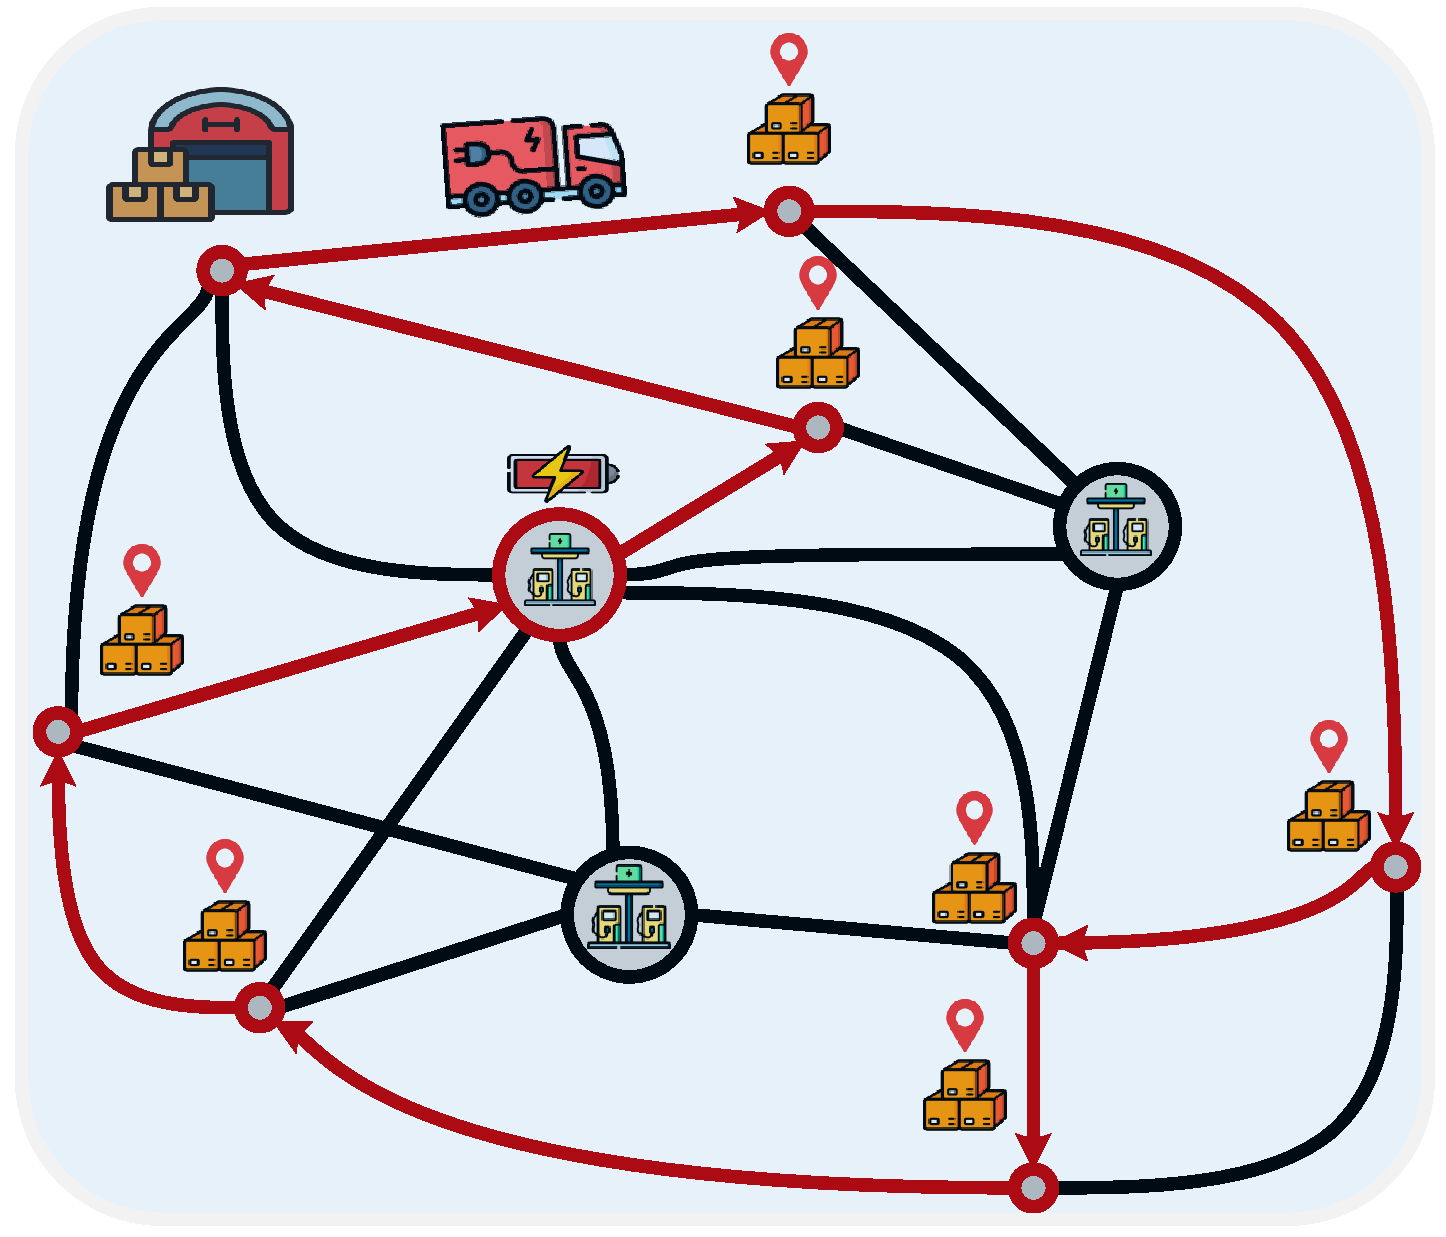
\includegraphics[width=0.4\linewidth]{TruckRoutingProblemOverview_a.pdf}
         \label{fig:ov_a}
         }
     \subfloat[Electric Truck Fleet Routing Problem]{
         \centering
         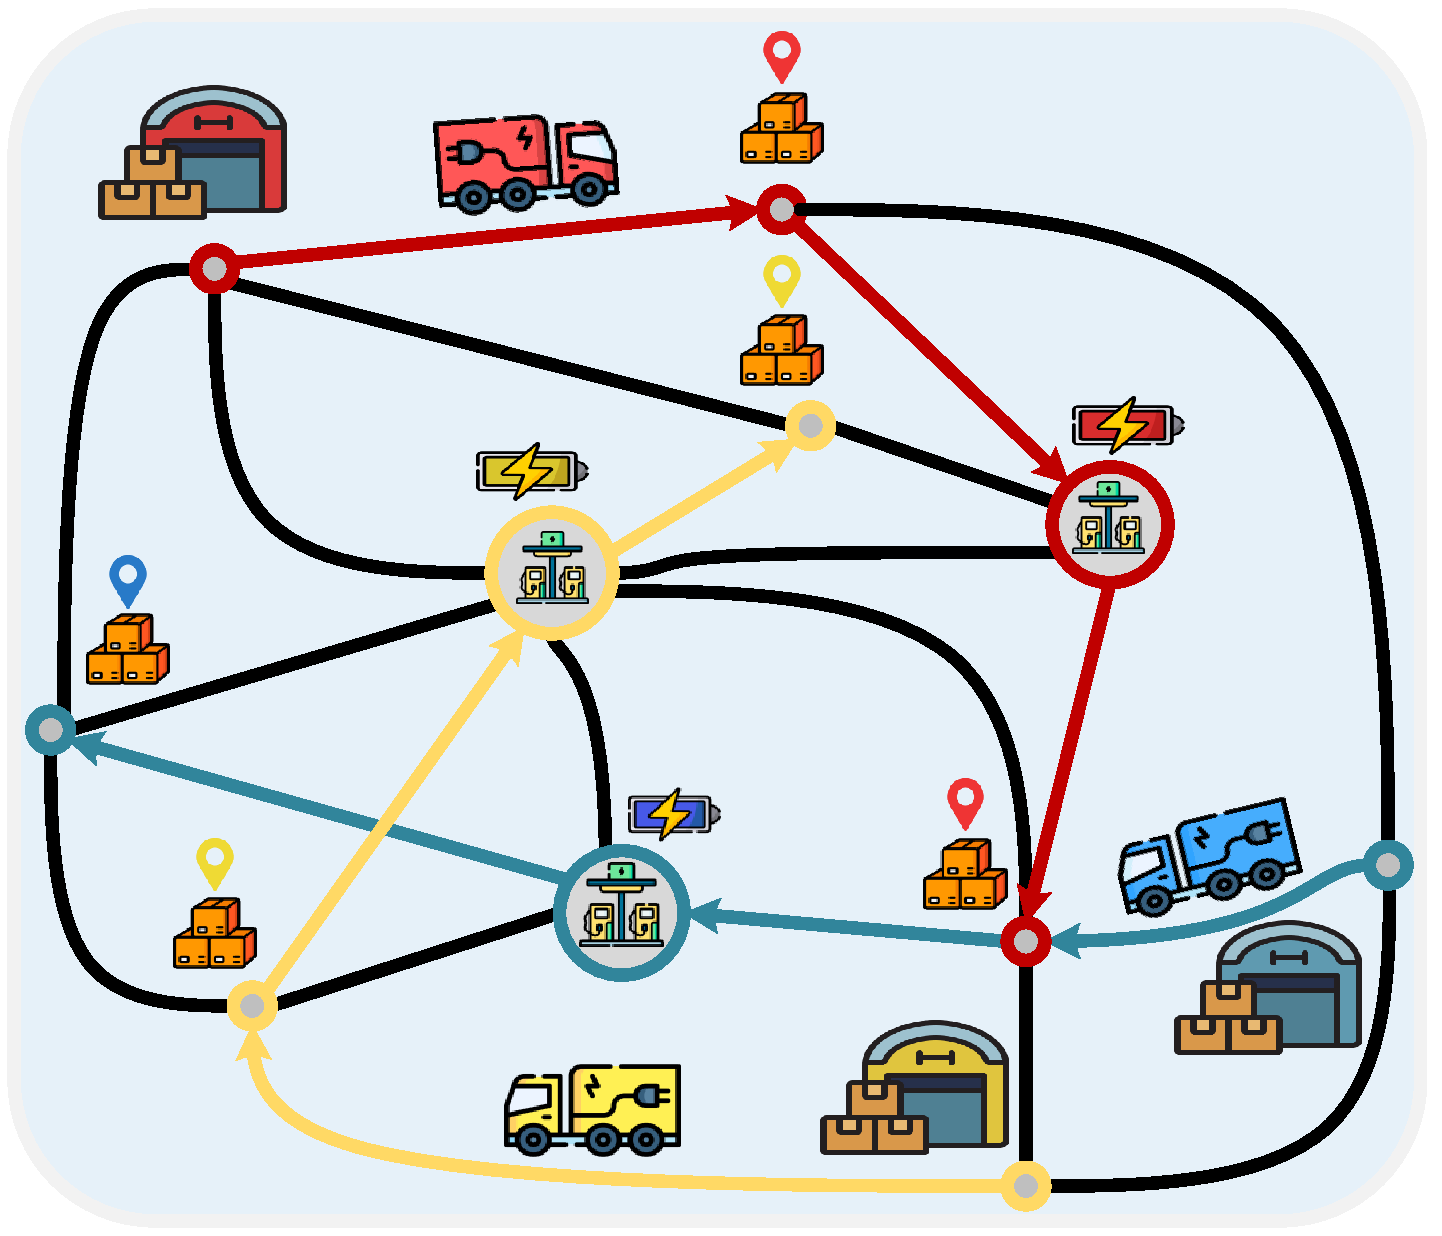
\includegraphics[width=0.4\linewidth]{TruckRoutingProblemOverview_b.pdf}
         \label{fig:ov_b}
         }
        \caption{Comparison of the classic eVRP and the eTFRP with shared charging resources. (a) In eVRP, routing is typically planned for a single vehicle (or independently across vehicles), where charging stops are inserted to maintain energy feasibility along a prescribed tour. (b) In eTFRP, multiple trucks operate concurrently and compete for limited charging capacity, so route execution is coupled through shared stations and potential queuing delays.
        }
        \label{fig:overview}
\end{figure}

\section{Event-Driven Truck State Machine}

\begin{figure}
    \centering
    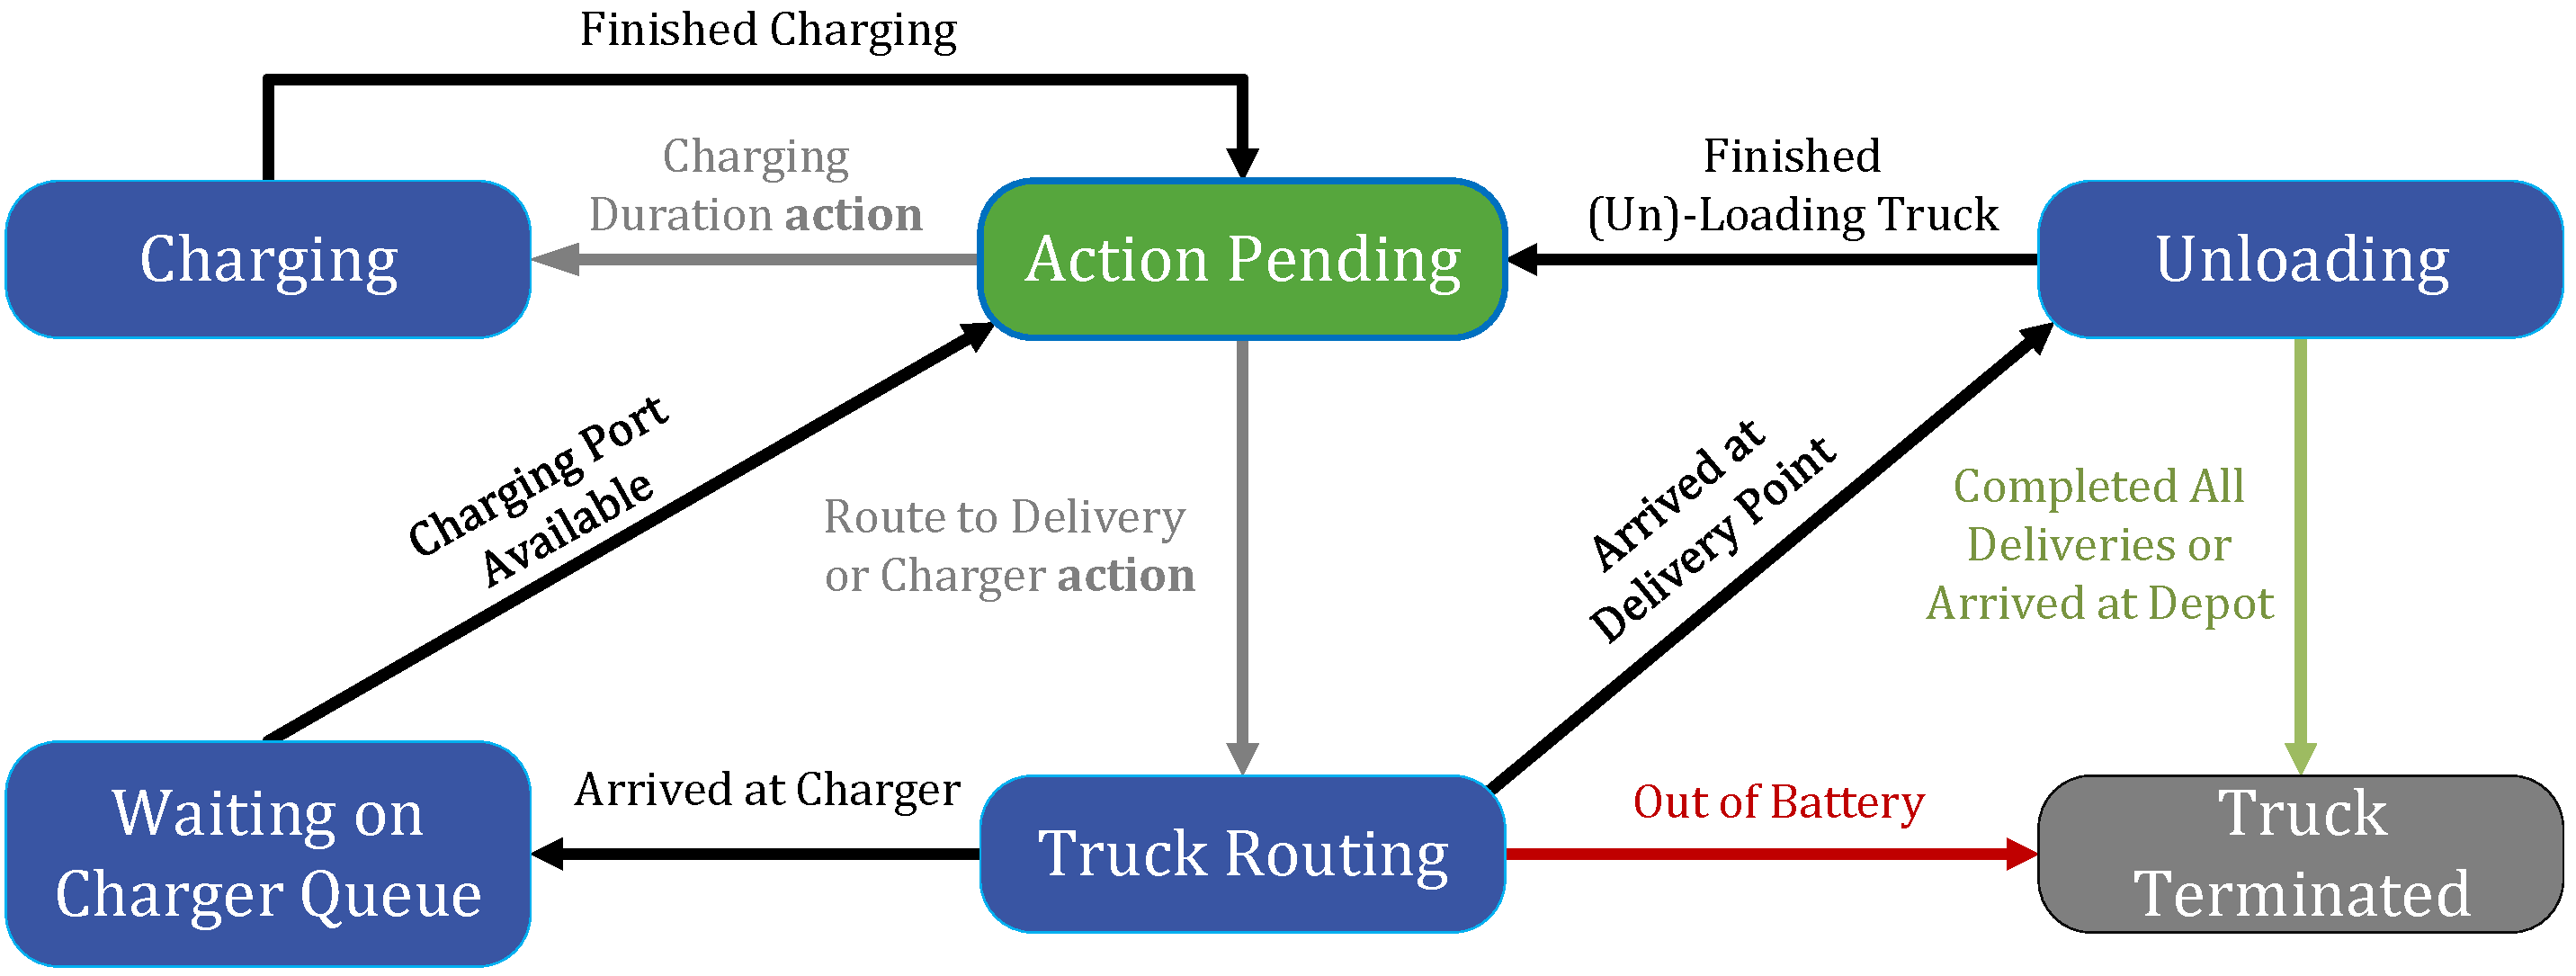
\includegraphics[width=0.8\linewidth]{TruckStateMachine_cropped.pdf}
    \caption{Event-driven truck state machine used by the simulator. Decision steps occur when a truck becomes \texttt{ready}; arrivals, charging, unloading, and FCFS (first-come, first-served) queuing trigger subsequent events.}
    \label{fig:truck_state_machine}
\end{figure}

\section{Linear Versus Tapered Fast-Charging Curves}

\begin{figure}
    \centering
    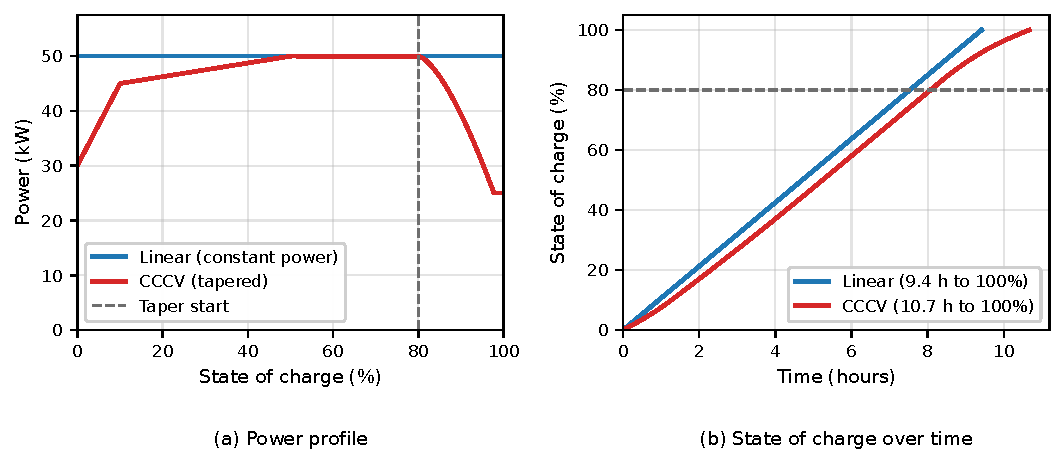
\includegraphics[width=0.75\linewidth]{charging_curve_comparison.pdf}
    \caption{Charging power profile and SoC evolution under constant-power (linear) charging versus tapered CCCV fast charging. Tapering reduces effective power at high SoC and changes optimal charging durations.}
    \label{fig:charging_curve}
\end{figure}

\section{Formulation Assumptions}\label{app:assumptions}

\begin{description}[leftmargin=*,nosep]
\item[Queueing.] Stations admit trucks first-come-first-served up to their port
count. Waiting time is endogenous: it depends on the fleet's own earlier
decisions, not on an exogenous draw. Joining the waiting list of a full station
is a legal routing decision rather than an error.
\item[Uncertainty.] Travel time, energy draw and service duration are drawn per
event from independent random streams keyed by the scenario seed, so a scenario
replays exactly. Energy is correlated with the realized travel time. Bounds are
given in Section~III of the main paper.
\item[Horizon and information.] The episode ends when every truck is complete or
failed, when the time limit is reached, or when no decision remains. Decisions
are taken at events, and the decision maker is centralized: it observes the
whole fleet and commits one action for the active truck.
\item[Fallback.] An action that the feasibility engine rejects is not silently
repaired. Under the default semantics it strands the truck and the episode
records the reason; under the variant used for the mask ablation it is refused
and charged a penalty. Every terminated or truncated episode carries a cause,
and failures are retained in every aggregate that is not explicitly conditioned
on success.
\end{description}

\section{Training Objective of GraphPPO}

The overall objective of RL~\cite{SuttonReinforcementIntroduction} is to find a stochastic policy $\pi_\theta(a\mid s)$ that maximizes the expected discounted return $r$ in the eTFRP, defined as
$J(\theta)\;\triangleq\;\mathbb{E}_{\pi_\theta}\!\left[\sum_{t=0}^{\infty}\gamma^{t}\,r_t\right]$, where $\gamma\in(0,1)$ is the discount factor. 
The critic network is trained on the one-step Bellman target $y_t = r_t + \gamma V_\phi(s_{t+1})$ with the loss $\mathcal{L}_V(\phi)=\mathbb{E}_t[(V_\phi(s_t)-y_t)^2]$. Using the standard PPO algorithm the advantages are estimated with generalized advantage estimation (GAE),
\begin{equation}
\widehat{A}_t 
\;=\;
\sum_{h=0}^{H-1}(\gamma\lambda)^h\,\big( r_{t+h} + \gamma\,V_\phi(s_{t+h+1}) - V_\phi(s_{t+h}) \big),
\label{eq:gae}
\end{equation}
where $\lambda\in[0,1]$ controls the bias--variance trade-off and $H$ is the rollout horizon.
Let $\theta_{\mathrm{old}}$ denote the parameters used to collect the rollout, and let $\rho_t(\theta)=\pi_\theta(a_t\mid s_t)/\pi_{\theta_{\mathrm{old}}}(a_t\mid s_t)$ be the importance ratio. GraphPPO then maximizes the clipped surrogate objective
\begin{equation}
\mathcal{L}^{\mathrm{PPO}}(\theta)
=\mathbb{E}_t\Big[
\min\big(\rho_t(\theta)\widehat{A}_t,\ \mathrm{clip}(\rho_t(\theta),1-\epsilon,1+\epsilon)\widehat{A}_t\big)
\Big],
\label{eq:ppo_objective}
\end{equation}
which prevents overly large policy updates by constraining $\rho_t(\theta)$ to a trust region of width $\epsilon$. In practice, the combined loss consists of the negative surrogate objective, the value regression loss, and an entropy bonus to encourage exploration.

\section{The GraphPPO Training Loop}

\begin{algorithm}[t]
\caption{GraphPPO}
\label{alg:vappo}
\begin{algorithmic}[1]
\State \textbf{Input:} discount $\gamma$, clip $\epsilon$, GAE $\lambda$, rollout length $L$, update epochs $E$
\State Initialize actor $\pi_\theta$ and critic $V_\phi$
\For{iteration $=1,2,\dots$}
    \State Set $\theta_{\mathrm{old}}\leftarrow \theta$; clear buffer $\mathcal{B}$
    \For{$t=0,\dots,L-1$}
        \State Observe state $s_t$ and feasible set $\mathcal{A}(s_t)$; build graphs $\mathcal{G}^{\mathcal{S}}_t$ and $\mathcal{G}^{\mathcal{A}}_t$
        \State Compute $\pi_{\theta_{\mathrm{old}}}(\cdot\mid s_t)$; sample $a_t\sim\pi_{\theta_{\mathrm{old}}}(\cdot\mid s_t)$; step env $\rightarrow (r_t,s_{t+1})$
        \State Store $(s_t,a_t,r_t,s_{t+1},\log\pi_{\theta_{\mathrm{old}}}(a_t\mid s_t))$ in $\mathcal{B}$
        \If{episode terminates} \textbf{break} \EndIf
    \EndFor
    \State Compute $\widehat{A}_t$ by GAE~\eqref{eq:gae} and value targets $y_t=r_t+\gamma V_\phi(s_{t+1})$
    \For{epoch $=1,\dots,E$}
        \State Sample minibatches from $\mathcal{B}$
        \State Update actor $\theta$ by maximizing PPO objective~\eqref{eq:ppo_objective} (plus entropy bonus)
        \State Update critic $\phi$ by minimizing $\mathbb{E}\big[(V_\phi(s_t)-y_t)^2\big]$
    \EndFor
\EndFor
\end{algorithmic}
\end{algorithm}

\section{Experimental Transportation Network}

\begin{figure}
  \centering
  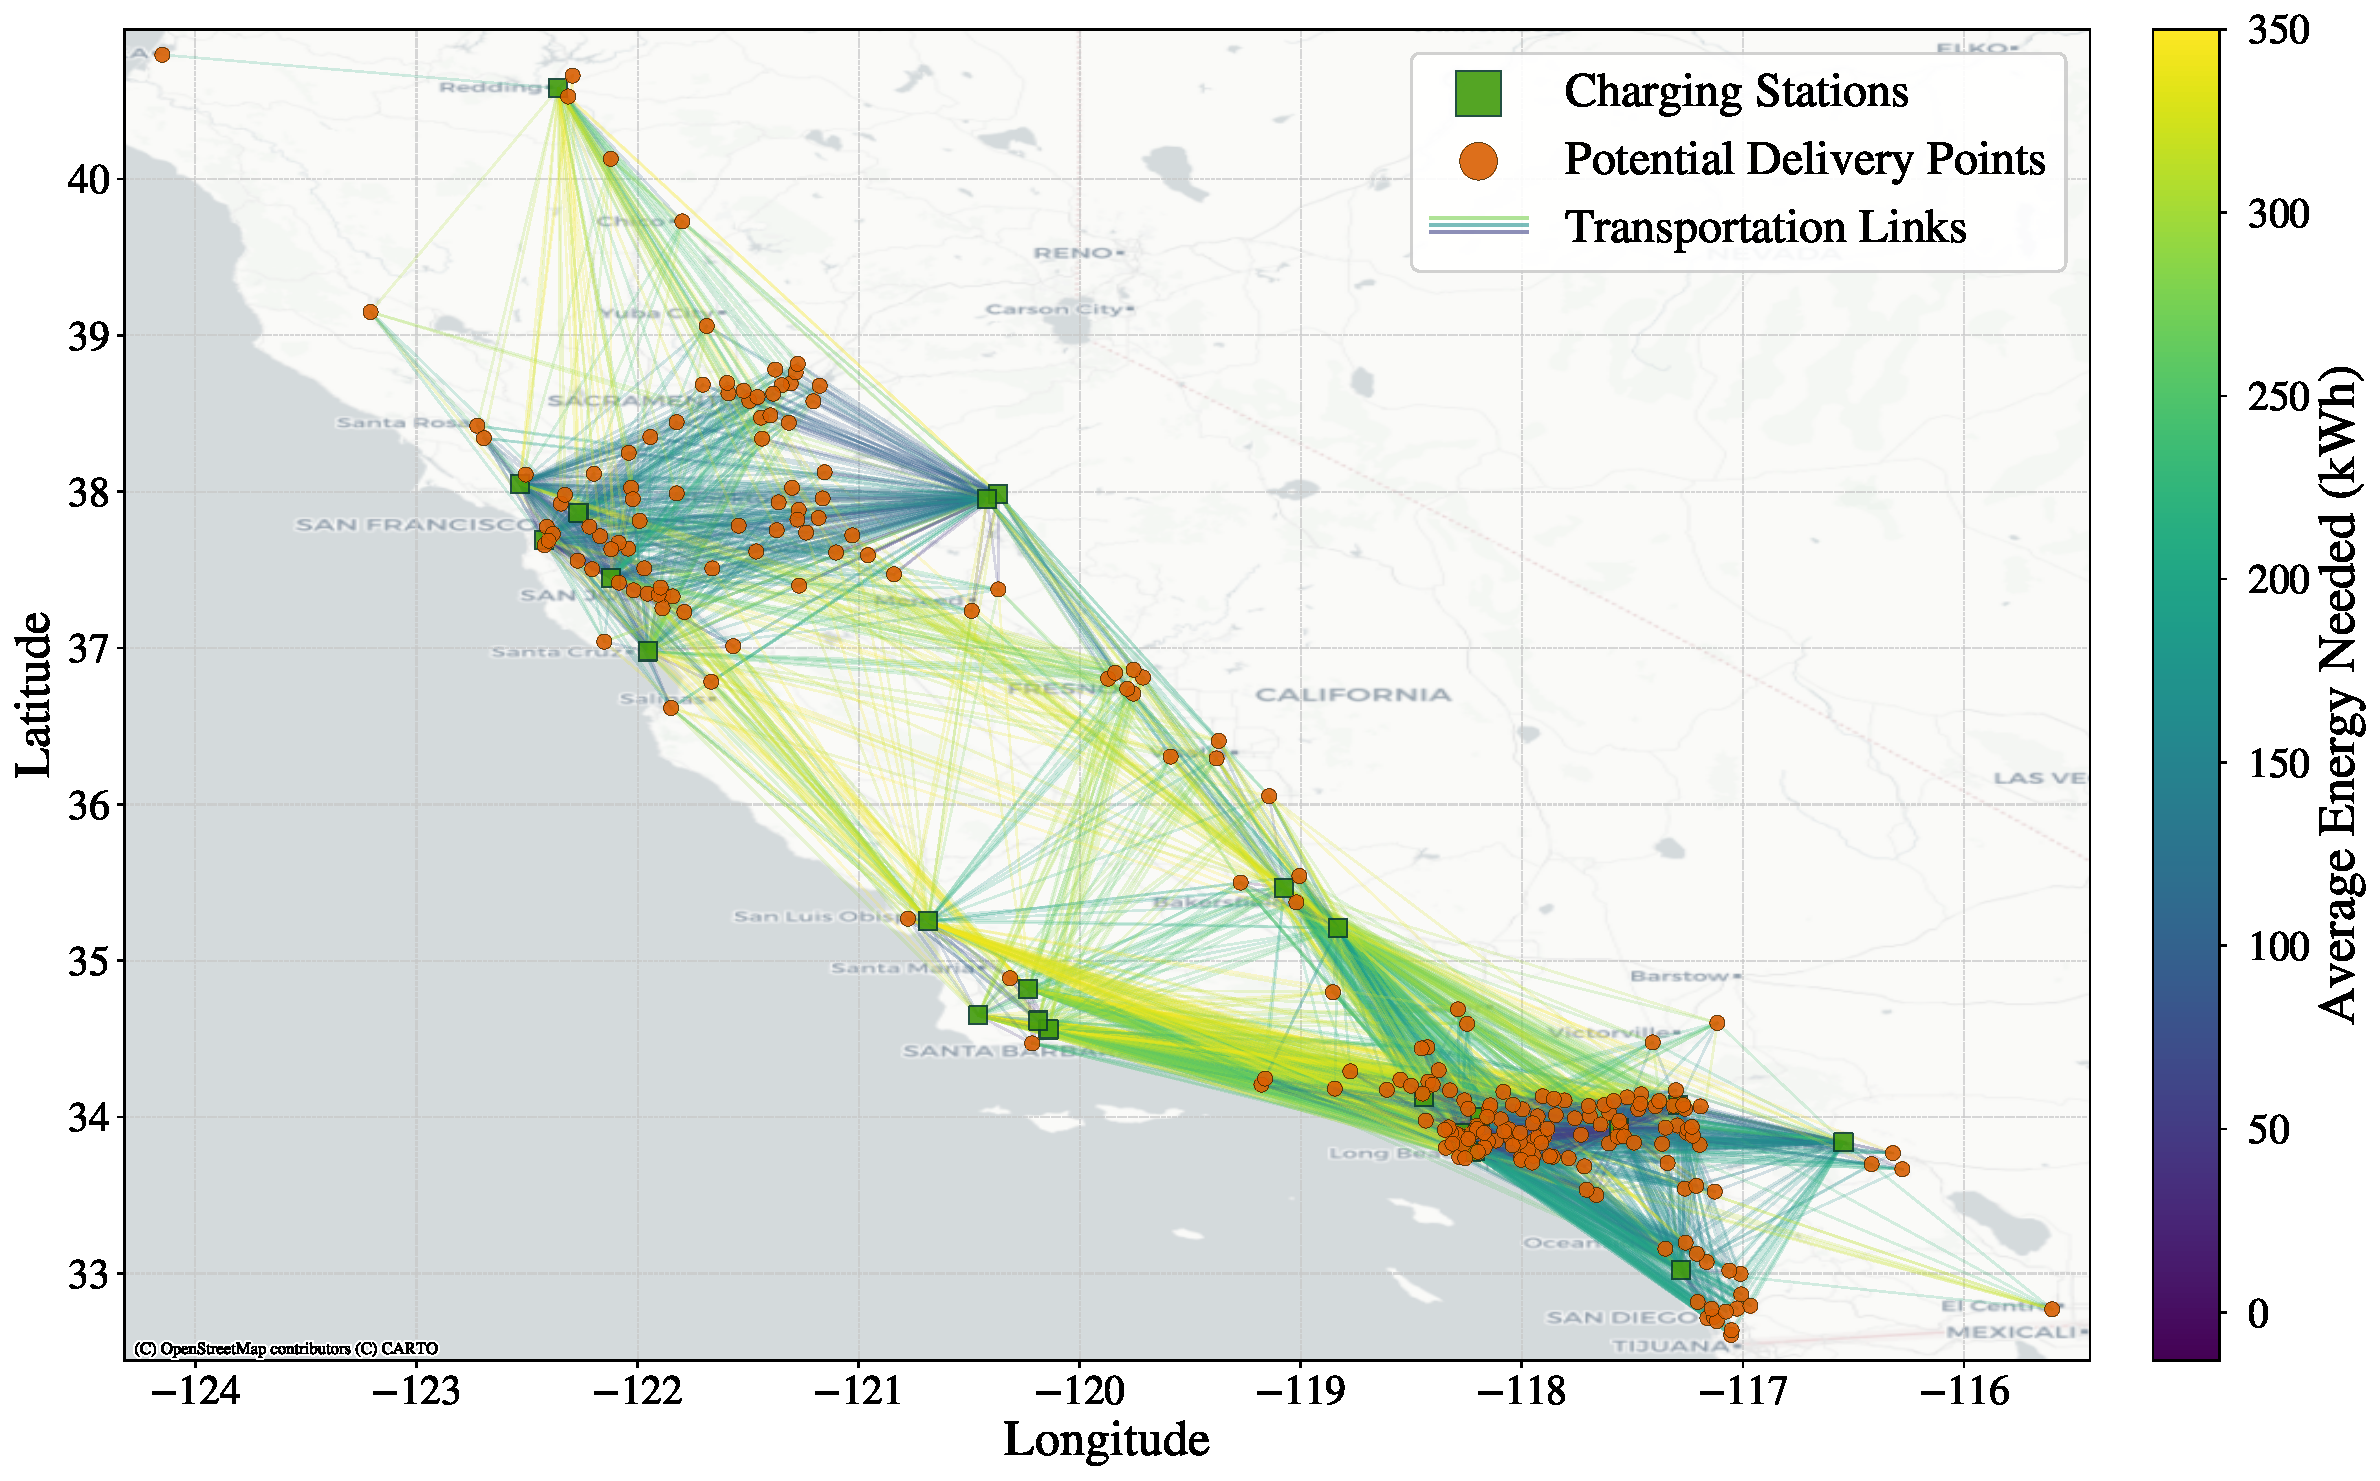
\includegraphics[width=0.75\linewidth]{transport_graph.pdf}
\caption{Experimental transportation network used in the case study. The figure shows the California transportation graph~\cite{ziyan2025} with sampled delivery locations and charging stations overlaid on the map. Node and edge colors indicate the spatial variation in energy and travel conditions across the network.}
\label{fig:cali}
\end{figure}

\section{Random Variables and Experimental Settings}

\begin{table}[t]
\centering
\caption{Random variables and experimental settings used in the routing environment. Untilded symbols denote nominal quantities and tilded symbols their realizations, and each entry states whether the quantity is drawn exogenously or arises endogenously from the fleet's own decisions.}
\label{tab:random_variables}
\small
\begin{tabular}{p{0.29\linewidth} p{0.60\linewidth}}
\toprule
\textbf{Random variable} & \textbf{Value / configuration} \\
\midrule
Travel time $\tilde{\tau}_{uv}(t)$
& $\tilde{\tau}_{uv}(t)\sim 
\mathcal{N}\!\left(\tau_{uv},\sigma_{uv}^{2}(t)\right)$; 
std.\ factor $0.15$, rush-hour multiplier $2.0$ \\

Realized edge energy $\tilde{b}_{uv}$
&
$\tilde{b}_{uv}=b_{uv}\,\xi_{uv}\in[0.90\,b_{uv},\,1.20\,b_{uv}]$, with
$\xi_{uv}=\operatorname{clip}\!\left(
1+0.5\!\left(\frac{\tilde{\tau}_{uv}}{\tau_{uv}}-1\right)
+\varepsilon_{uv},\,0.90,\,1.20
\right)$, $\varepsilon_{uv}\sim\mathcal{N}\!\left(0,0.05^{2}\right)$;
correlated with travel time through $\tilde{\tau}_{uv}/\tau_{uv}$ \\

Charging action
& Target state of charge $\in\{0.5,0.6,0.7,0.8,0.9,1.0\}$; the realized
duration follows from the charging curve \\

Charging model
& CCCV enabled; station classes $\{150,350,750\}$ kW, $\eta_c=0.90$,
taper from SoC $0.8$ down to $150$ kW \\

Queueing time
& Endogenous: FCFS admission at finite ports, so waiting depends on the
fleet's own prior decisions rather than on an exogenous draw \\

Unloading time $\tilde{q}$
& Base $0.2$ h, sampled once per service event; std.\ factor $0.20$,
capped at $0.25$ h, $1.5\times$ during business hours \\

Initial battery
& Full battery; $\overline{b}_i=400$ kWh \\
\bottomrule
\end{tabular}
\end{table}

\section{Evaluation Protocol for the Joint Fleet eVRP Study}

The joint fleet eVRP study of Section~V-C of the main paper follows a separate and stricter protocol, which we state here because it governs every number in Sections~V-C to V-E of the main paper. Scenario seeds are drawn from provably disjoint train, validation, and test namespaces. All baseline hyperparameters and all checkpoint selections are made on validation scenarios only, under a pre-declared rule, and no test scenario is read until the frozen method set is scored. Ablation arms are re-scored on validation scenarios beyond those used to select their own checkpoints, so a comparison between arms is independent of the selection that produced them. Each evaluated method publishes an immutable manifest recording the resolved configuration, the seed list, the code revision, and the checkpoint, together with per-episode rows that retain failures and record their cause; aggregate figures conditioned on success state the conditioning explicitly.

Two consequences of this protocol should be read alongside the results. First, because independently seeded runs of the identical configuration differ by up to $0.107$ in success rate at the interaction budget used for the ablations, differences smaller than roughly $0.1$ are reported as indistinguishable from training noise rather than interpreted. Learned entries in Table~II of the main paper therefore give a seed range where three seeds were trained and are marked as single-seed otherwise. Second, the optimization baseline used in that study is a fleet-level CP-SAT model whose nominal objective was checked against exhaustive enumeration on instances small enough to enumerate; it agrees with brute force on all of them, as does the ALNS metaheuristic, so the planners' shortfall in the stochastic setting reflects open-loop execution rather than an inability to solve the nominal problem.

\section{Baseline Specifications and Information Assumptions}\label{app:baselines}

This appendix states what each non-learning baseline knows, what it assumes, and
what it does when its plan fails, so that the comparison in
Section~V-C of the main paper can be reproduced or disputed on its details rather
than on its summary.

\subsection*{A.1 Information available to every method}

All methods, learned and classical, observe the same state: the position,
battery, remaining payload and status of every truck; the location, demand and
service status of every customer; the location, power, port count, occupancy and
waiting list of every station; and the nominal travel time and energy of every
network transition. No method observes a realized travel time, energy draw or
service duration before it is incurred, and no method observes another truck's
future decisions. The nominal network is the same table for all methods and is
never perturbed by the realizations drawn during an episode.

\subsection*{A.2 Greedy heuristic}

The heuristic is goal-directed rather than myopic, and three properties were
necessary to make it a fair opponent rather than a straw man; each is stated
because each corresponds to a failure mode we measured.

\begin{enumerate}[leftmargin=*,nosep]
\item \textbf{Charger choice must close distance to the goal.} Selecting the
nearest station makes trucks shuttle between two adjacent stations indefinitely
when a customer lies more than one battery away.
\item \textbf{A stop is only taken if the truck can also leave it.} Serving a
customer the truck cannot depart from strands it, because the episode requires a
depot return.
\item \textbf{Customers claimed by another truck are excluded.} They are
permanently infeasible for this truck, and targeting them wastes decisions.
\end{enumerate}

\noindent The resulting policy is, at each decision point for the active truck
$i$ at node $n_i$:

\begin{quote}
\small
\textbf{if} a delivery is in progress or the truck must leave a charger:
  take the forced transition.\\
\textbf{else} let $G$ be the set of unserved customers claimable by $i$ within
its remaining payload, plus the depot if all customers are served.\\
\quad Choose the goal $g\in G$ minimising
$\tau_{n_i g} + w\cdot d_g$, where $d_g$ is the customer's demand and $w$ the
demand weight.\\
\quad \textbf{if} $\alpha\cdot b_{n_i g} \le$ battery and the truck can also
leave $g$: drive to $g$.\\
\quad \textbf{else} choose the station $c$ minimising
$\tau_{n_i c} + \tau_{c g}$ among stations reachable with the energy margin
$\alpha$, and drive to $c$; on arrival, charge to the target state of charge.
\end{quote}

\noindent Here $\alpha$ is the energy safety factor. Recharge duration is priced
with the same nonlinear charging routine the simulator executes, not with an
energy-over-power approximation, so the heuristic never plans a recharge the
simulator will not deliver. Parameters ($\alpha$, target state of charge, demand
weight) are grid-searched on validation scenarios only.

\subsection*{A.3 Rolling-horizon controller}

The controller enumerates sequences of the next $H$ stops with branching factor
$B$ over the nominal network, scores each by its nominal completion time with
energy-safe recharges inserted, commits only the first stop, and re-plans at the
next decision point. It is therefore deterministic and receding-horizon: it uses
expected values for travel and energy and never samples scenarios. It executes
through the heuristic's navigation layer, so a failure to reach a planned stop
is repaired rather than propagated.

\subsection*{A.4 CP-SAT planner}

The planner solves the nominal deterministic problem once per scenario: a
circuit formulation per truck over the depot and all unserved customers, with
payload capacity enforced, arc costs equal to nominal travel time plus the
recharge time that arc's energy implies at an average charging power, and an
objective of either the longest route or the sum of routes. It is offline and
deterministic; it does not model queueing, does not sample realizations, and
does not re-solve when execution departs from the plan. Execution uses the same
energy-safe navigation layer, and every episode records how often the plan ran
out and the executor chose instead.

Two properties matter for interpreting the results. First, the circuit admits an
empty route, so a truck may be left idle; without this the model is forced to
use every vehicle and returns strictly worse plans while reporting them as
optimal. Second, the objective is validated: on instances small enough to
enumerate, the solved objective matches exhaustive enumeration over all
assignments and orderings.

\subsection*{A.5 Adaptive large neighbourhood search}

ALNS searches the same nominal objective as the CP-SAT planner. It begins from a
cheapest-insertion construction and repeats: remove a fraction of customers with
one of four destroy operators (random, worst-cost, Shaw-related, whole-route),
reinsert them with greedy or regret-2 insertion, and accept by a
simulated-annealing criterion. Operator weights adapt on the standard
Ropke--Pisinger schedule. The search is deterministic given its seed, and it
executes through the same navigation layer as the other planners. It reports no
optimality bound by construction.

\section{Episode-Wise Win Rates Across eTFRP Settings}

\begin{figure}
  \centering
  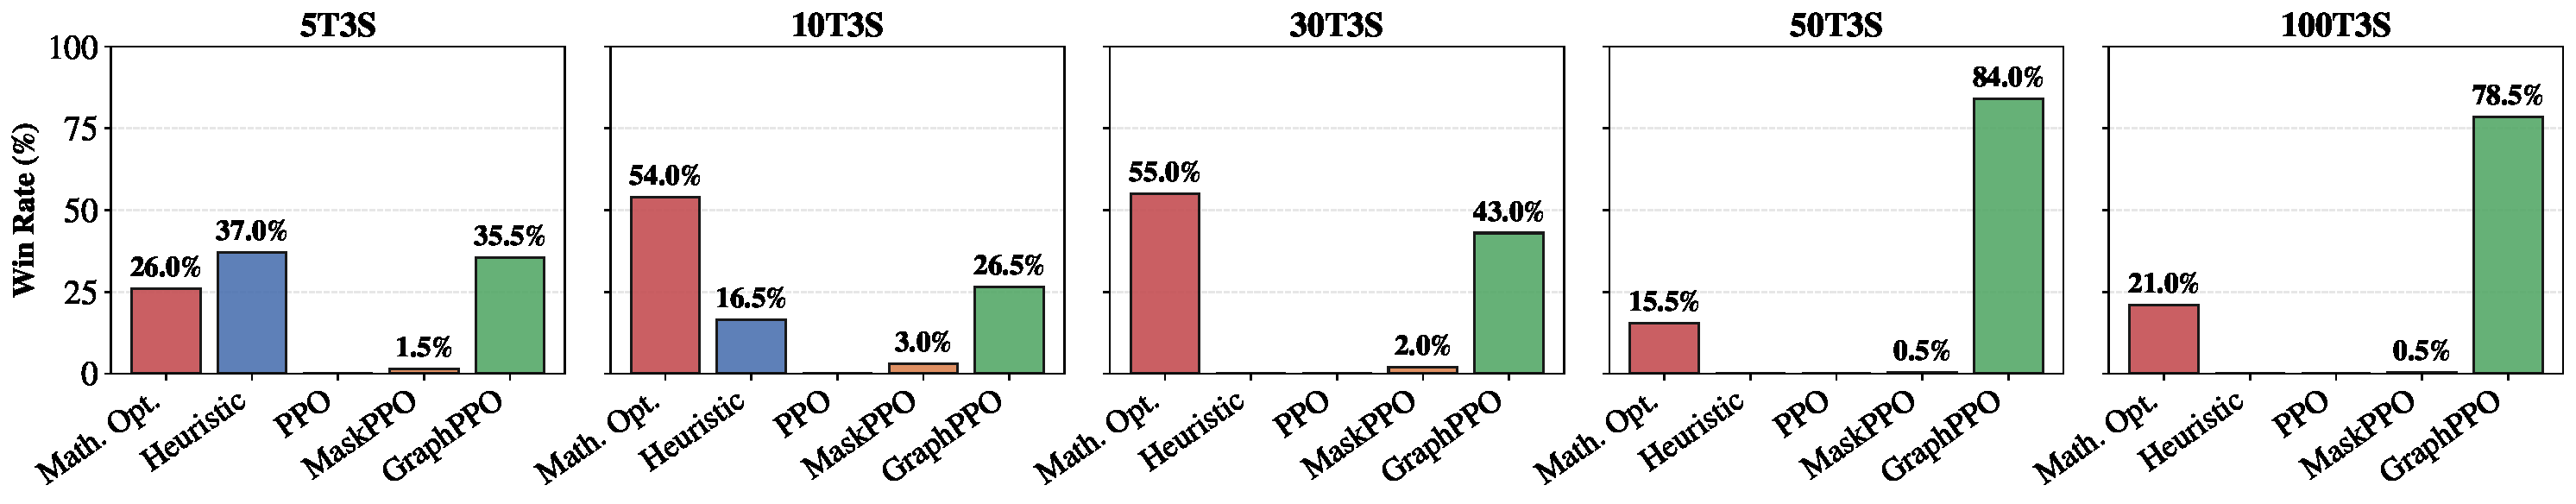
\includegraphics[width=1\linewidth]{win_rates.pdf}
\caption{Comparison of episode-wise winning frequency across 200 simulation episodes for different eTFRP settings. Each bar shows the percentage of episodes in which a method produced the best-performing solution among the compared methods.}
\label{fig:wr}
\end{figure}

\section{Generalization from a Single Training Setting}

\subsection{Generalization from a Single Training Setting}

\begin{figure} 
\centering
     \subfloat[Normalized reward ratio]{
         \centering
         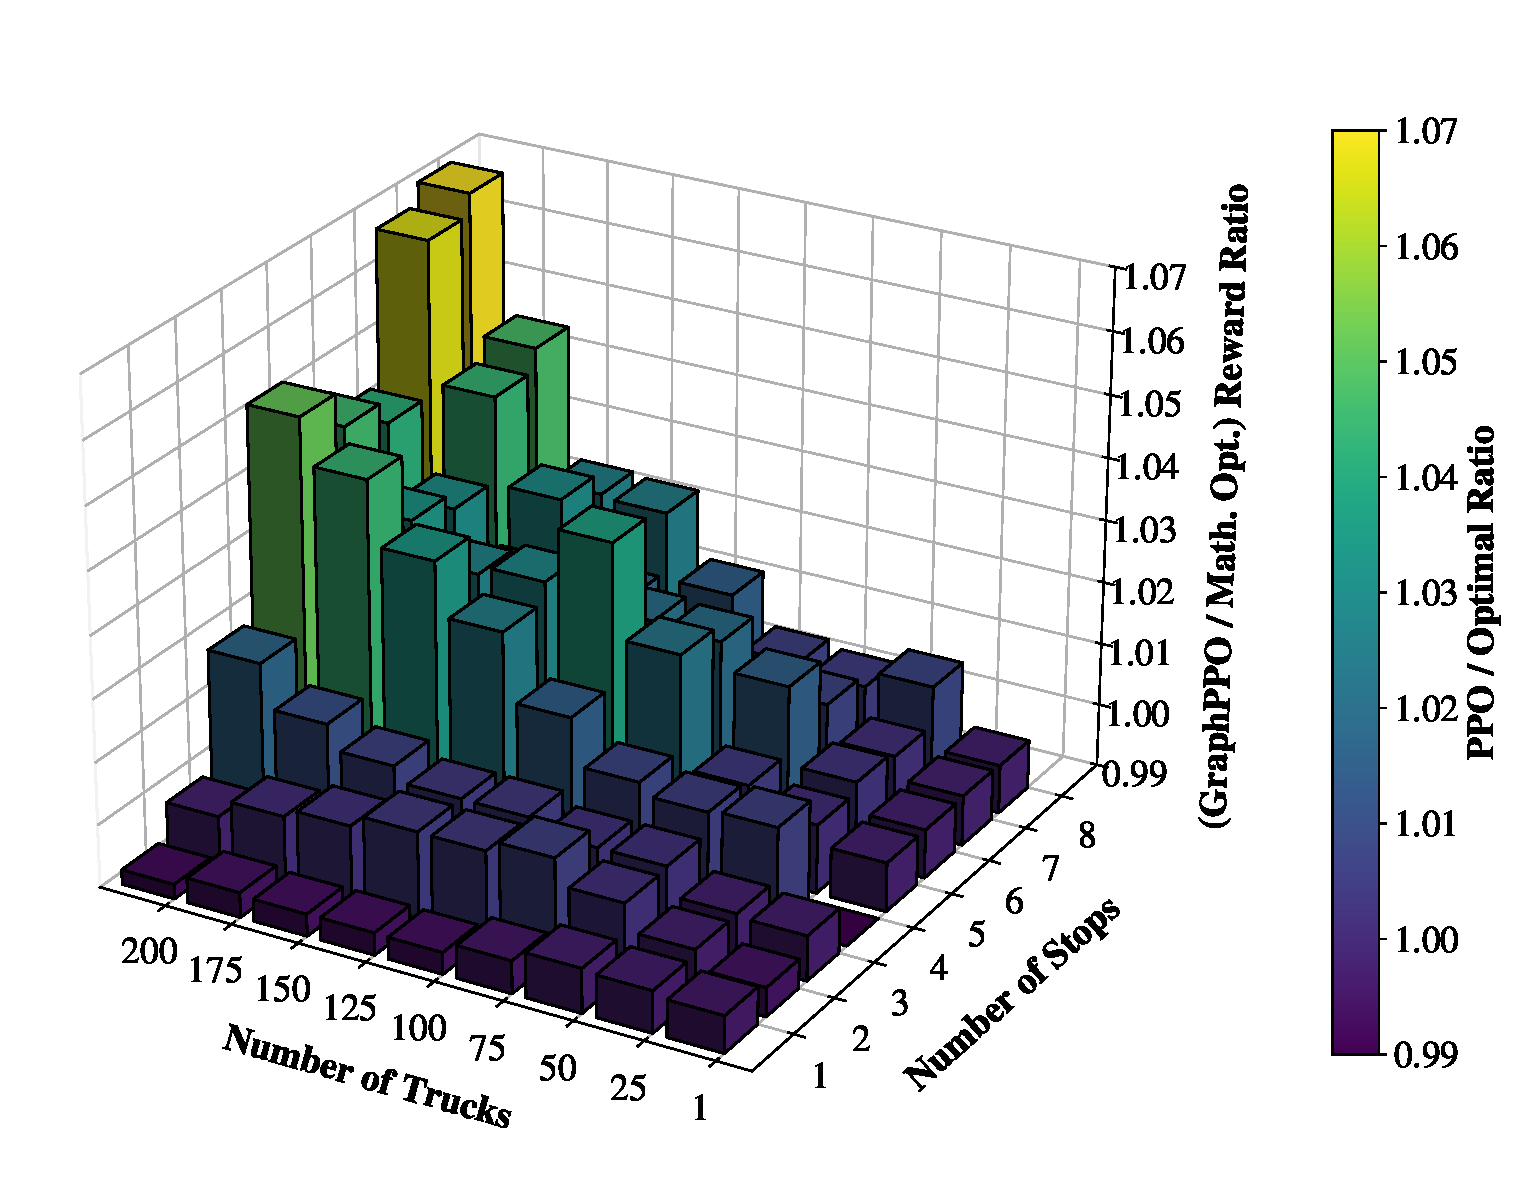
\includegraphics[width=0.4\linewidth]{grid_eval_3d_ratio_plot.pdf}
         \label{fig:gen_a}
         }
        \hspace{10mm}
     \subfloat[Win ratio]{
         \centering
         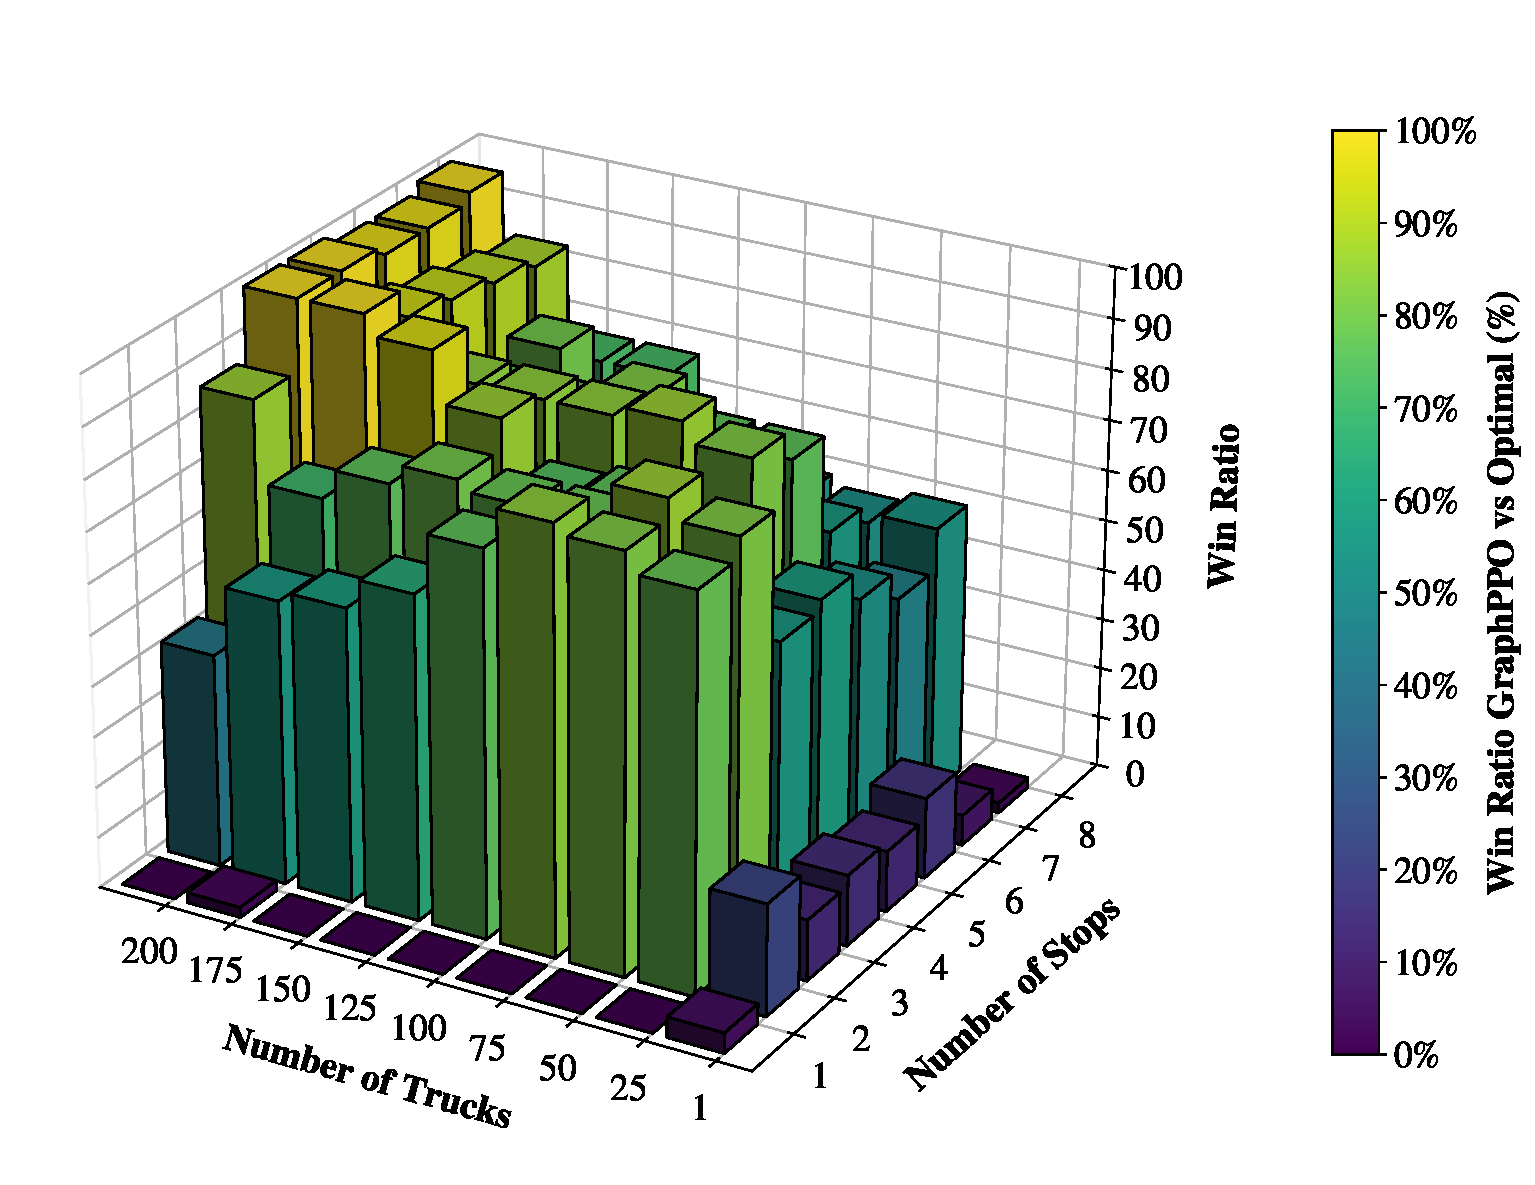
\includegraphics[width=0.4\linewidth]{grid_eval_3d_ratio_plot_win_ratio.pdf}
         \label{fig:gen_b}
         }
    \caption{Generalization performance of a GraphPPO policy trained only on the 100T3S setting and evaluated without retraining across different eTFRP configurations, averaged over 50 random scenarios per case. Panel (a) reports the normalized reward ratio relative to Math.\ Opt., while panel (b) reports the win ratio against Math.\ Opt., defined as the percentage of scenarios in which GraphPPO achieves the better outcome.}
        \label{fig:gen}
\end{figure}


A \emph{size-transfer} analysis is conducted in Figure~\ref{fig:gen}, where a single GraphPPO policy trained only on the 100T3S setting is applied directly to all other fleet-size and stop-count configurations without any retraining or fine-tuning. The transfer examined here is deliberately narrow: the generator, the road network, the vehicle parameters, and the uncertainty law are all held fixed, and only the instance size changes. It is therefore evidence of transfer across scale, not of out-of-distribution generalization; the latter is examined separately in Section~V-C of the main paper, where the charging infrastructure, battery capacity, service times, road distances, and uncertainty distributions are each shifted in turn. The horizontal axes span the number of trucks and the number of sequential stops per truck, while each reported value is averaged over 50 random scenarios. Two complementary metrics are shown. Panel~(a) reports the normalized reward ratio, defined as the average GraphPPO reward divided by the average reward of Math.\ Opt.\ for the same setting, so values above $1.0$ indicate that the transferred policy outperforms the conservative optimization benchmark on average. Panel~(b) reports the win ratio against Math.\ Opt., i.e., the percentage of scenarios in which GraphPPO achieves a better outcome than the optimization benchmark.

Strong transfer performance is observed over a broad region of the test space. In panel~(a), the normalized reward ratio remains very close to or above parity in almost all settings, typically lying around $1.00$ to $1.04$, while the strongest gains are obtained in larger and more congested instances, where values rise to approximately $1.06$ to $1.07$. The largest advantage is visible in high-truck and mid-to-high stop settings, especially around 150 to 200 trucks and roughly 5 to 7 stops, indicating that the policy learned on 100T3S captures decision patterns that remain effective as congestion and fleet interactions become even stronger.
At the same time, only limited degradation is observed in smaller settings. A likely explanation is that instances with few trucks or stops offer relatively little variability in feasible solutions, making the decision landscape simpler. Consequently, the reward ratio remains close to 1.0, suggesting that the learned policy does not over-specialize to the training configuration.

The win-ratio results in panel~(b) further support this conclusion, although a more heterogeneous pattern is observed because this metric is stricter than average reward comparison. For medium and large fleets with approximately 2 to 6 stops, GraphPPO wins in a large majority of scenarios, with win ratios often between $70\%$ and $100\%$, and with the highest values appearing in the dense multi-truck regimes where charger competition is strongest. By contrast, the smallest instances and the one-stop cases are associated with much lower win ratios, in some cases close to zero, indicating that the optimization benchmark remains more competitive when the problem structure is simple, and congestion at charging stations is limited. Overall, the results indicate that the policy trained on 100T3S generalizes well across both smaller and larger eTFRP settings, with the most substantial advantage retained in the operational regimes most relevant to large-scale fleet coordination.


\section{In-Depth Analysis for a Single Setting}

\subsection{In-Depth Analysis for a Single Setting}

A more detailed comparison is provided through the representative 10T3S setting, which corresponds to 10 trucks and 3 sequential delivery stops per truck, while all reported values in Table~\ref{tab:10t3s_metrics} are averaged over 200 evaluation scenarios and are shown as mean $\pm$ standard deviation.

The 10T3S setting is selected as a representative benchmark because it strikes a balance between problem complexity and computational tractability. With 10 trucks and 3 sequential delivery stops per truck, the setting introduces sufficient combinatorial diversity to meaningfully evaluate the model's decision-making capabilities while remaining interpretable for detailed analysis.
Table~\ref{tab:10t3s_metrics} shows detailed results averaged over 200 evaluation scenarios.
The reported {Reward} corresponds to the episodic return used by the environment, which jointly reflects routing, charging, waiting, unloading, successful delivery, and failure penalties. The {Success Rate} indicates the percentage of scenarios completed feasibly. The {Avg.\ Truck SoC at Finish} measures the average remaining battery level at the end of the episode, while {Total Deliveries} reports how many deliveries are completed across the fleet. The charging-related indicators are separated into {Total Charging Sessions}, which counts the number of charging actions; {Total Charging Time}, which measures the aggregate time spent charging, and {Total Waiting Time}, which captures the time spent in charger queues. In addition, {Total Routing Time} and {Unloading Time} quantify time spent traveling and servicing deliveries, {Total Time} summarizes the overall operational duration, and Exec.\ Time reports the wall-clock solution time required by each method.


\begin{table*}[t]
\centering
\small
\caption{Detailed metric performance comparison for the 10T3S setting over 200 evaluation scenarios. Reported values are the mean and standard deviation over the evaluation scenarios.}
\begin{tabular}{@{}lccccc@{}}
\toprule
Metric & Math. Opt. & Heuristic & PPO & MaskPPO & GraphPPO (Ours) \\
\midrule
Reward (-) & $14582$ $\pm$ $583$ & $11718$ $\pm$ $2245$ & $1244$ $\pm$ $2205$ & $14404$ $\pm$ $721$ & $14574$ $\pm$ $568$ \\
Success Rate (\%) & $95.5$ $\pm$ $20.8$ & $16.5$ $\pm$ $37.2$ & $0.0$ $\pm$ $0.0$ & $87.5$ $\pm$ $33.2$ & $95.0$ $\pm$ $21.8$ \\
Avg. Truck SoC at Finish (\%) & $36.0$ $\pm$ $3.4$ & $14.6$ $\pm$ $6.4$ & $27.0$ $\pm$ $6.4$ & $50.1$ $\pm$ $7.1$ & $14.2$ $\pm$ $2.4$ \\
Total Deliveries (-) & $29.9$ $\pm$ $0.7$ & $27.4$ $\pm$ $2.2$ & $19.4$ $\pm$ $2.3$ & $29.7$ $\pm$ $0.9$ & $29.9$ $\pm$ $0.6$ \\
Total Charging Sessions (-) & $13.5$ $\pm$ $1.8$ & $9.2$ $\pm$ $2.0$ & $0.0$ $\pm$ $0.0$ & $11.4$ $\pm$ $5.3$ & $13.5$ $\pm$ $2.6$ \\
\midrule
Total Charging Time (H) & $63.1$ $\pm$ $10.0$ & $28.4$ $\pm$ $7.7$ & $0.0$ $\pm$ $0.0$ & $87.8$ $\pm$ $19.0$ & $48.6$ $\pm$ $12.3$ \\
Total Waiting Time (H) & $4.3$ $\pm$ $8.2$ & $0.7$ $\pm$ $2.0$ & $0.0$ $\pm$ $0.0$ & $5.4$ $\pm$ $9.0$ & $2.0$ $\pm$ $3.7$ \\
Total Routing Time (H) & $224.3$ $\pm$ $16.6$ & $207.8$ $\pm$ $20.3$ & $132.5$ $\pm$ $12.7$ & $246.7$ $\pm$ $29.6$ & $249.6$ $\pm$ $23.2$ \\
Unloading Time (H)& $4.0$ $\pm$ $0.1$ & $3.8$ $\pm$ $0.2$ & $3.5$ $\pm$ $0.3$ & $4.0$ $\pm$ $0.1$ & $4.0$ $\pm$ $0.1$ \\
Total Time (H) & $295.8$ $\pm$ $27.3$ & $240.7$ $\pm$ $26.9$ & $136.0$ $\pm$ $12.9$ & $343.9$ $\pm$ $48.0$ & $304.1$ $\pm$ $35.0$ \\
\midrule
Exec. Time (s) & $1.9$ $\pm$ $0.7$ & $0.1$ $\pm$ $0.1$ & $0.2$ $\pm$ $0.2$ & $1.0$ $\pm$ $0.7$ & $1.7$ $\pm$ $0.3$ \\
\bottomrule
\end{tabular}
\label{tab:10t3s_metrics}
\end{table*}

For this case, near-equivalence between GraphPPO and the mathematical benchmark is observed in the two most important outcome metrics. A reward of $14574$ is obtained by GraphPPO, compared with $14582$ for Math.\ Opt., while the success rate remains almost identical at $95.0$ versus $95.5$. A comparable number of deliveries is also completed, with both methods averaging $29.9$ deliveries, and an identical average number of charging sessions is recorded at $13.5$. These results indicate that the proposed policy reproduces the overall quality and feasibility of the optimization benchmark under stochastic execution. By contrast, substantial degradation is observed for the heuristic and PPO baselines. The heuristic reaches a reward of $11718$ with only $16.5\%$ success, while generic PPO collapses completely with $0.0\%$ success and only $19.4$ completed deliveries. MaskPPO remains much stronger than PPO, with a reward of $14404$ and success of $87.5\%$, but still remains below both Math.\ Opt.\ and GraphPPO in reliability.

The operational metrics further clarify the behavioral differences among methods. GraphPPO ends with a lower residual SoC than Math. Opt.\ at $14.2\%$ versus $36.0\%$, which suggests that less conservative battery utilization is being adopted while feasibility is still preserved. This behavior is also reflected in the charging profile, since GraphPPO spends only $48.6$ hours in charging compared with $63.1$ for Math. Opt., and queueing time is reduced from $4.3$ hours to $2.0$ h. At the same time, a longer routing time is observed for GraphPPO at $249.6$ hours versus $224.3$, so the final total time is slightly higher at $304.1$ hours compared with $295.8$. A different pattern is observed for MaskPPO, where a very high terminal SoC of $50.1\%$ is retained together with $87.8$ hours of charging time and $343.9$ hours of total time, indicating an overly conservative charging strategy. Finally, low online solution times are maintained by all methods, with $1.7$ seconds for GraphPPO and $1.9$ seconds for Math.\ Opt. (since there are only 10 trucks), while the heuristic and PPO-based baselines remain below one second, so near-real-time deployment remains feasible for the proposed policy in this setting.


\section{Component Sweep of the Proposed Representation}

Three elements are found to carry the model. Removing the per-action routing features, which price the leg a candidate commits to and the return leg it implies, reduces the success rate from the $0.700$--$0.807$ seed band to $0.213$. Removing the typed pairwise relations between trucks, customers, and chargers reduces it to $0.633$, and withholding the pooled fleet embedding from the action head reduces it to $0.667$. Two elements are found to be inert: blanking the charging-queue state leaves the model at $0.793$ and blanking the active-truck indicator leaves it at $0.727$, both within the seed band. The queue result is a property of the evaluated instances rather than of the architecture, since two trucks distributed over twenty-five stations rarely contend for ports; a congestion-specific study is therefore required before any claim about queue-aware behaviour is made.

\section{Cost of Infeasibility Versus the Feasibility Mask}

What proves necessary is that infeasibility carry a cost commensurate with failure. When an infeasible action is merely refused at a tenth of the failure penalty, the policy never learns feasibility at all and the success rate collapses to zero; when the same refusal is charged at the failure penalty, the arm recovers to $0.773$. The mask is best understood as a convenience that supplies this cost for free, rather than as the source of the reported behaviour.
\section{Additional Ablations}

The same ablation was repeated in a pre-assigned variant of the problem, in which customers are bound to
trucks before the episode begins as they are in the eTFRP benchmark, so that only sequencing, charging and routing
remain to be decided. Across two seeds per arm the masked and unmasked policies reach $0.340$ and $0.330$ mean
success, against per-arm seed ranges of $0.054$ and $0.034$: the conclusion is unchanged in the setting the main
benchmark uses. This also locates what the earlier PPO-versus-MaskPPO comparison measures. Those two baselines differ
in their action representation as well as in masking, so their gap is evidence for the structured action space rather
than for the mask specifically.

A second observation from that variant is worth recording because it runs against intuition. At an identical budget
and architecture the same model reaches $0.70$--$0.81$ success when it also decides the assignment, and only
$0.31$--$0.37$ when the assignment is fixed. Removing a decision did not make the problem easier: under
pre-assignment a truck must serve its own customers wherever they fall, so the fleet cannot rebalance when one truck
draws a distant or energy-expensive set, and a customer that becomes unreachable stays unreachable. Assignment is not
only a decision the eTFRP removes; it is also the mechanism by which the joint formulation recovers from an adverse
draw.

The charging action space is examined in the same way. Refining the target state-of-charge grid from $10\%$ to $5\%$ leaves the model inside its seed band, so the coarser discretization is not a binding approximation. Expressing the charging decision as a duration of $15$, $30$, or $60$ minutes instead of a target state of charge reduces success to $0.627$ and increases fleet travel time to $159.3$ hours, placing it outside the band on both axes. The explanation is structural: a fixed duration delivers different amounts of energy depending on the truck's position on the charging curve, so the same action denotes different outcomes in different states, whereas a target state of charge is state-independent by construction.

{\footnotesize
\bibliographystyle{IEEEtranN}
\bibliography{ref}
}

\end{document}
